% \chapter{Deployment view (UML Deployment diagram)}\label{ch:deployment}

% Delete the command below to remove the hints and instructions
\showdeploynotes{}

\section{Context diagram}
    The context diagram for the deployment view is displayed in figure \ref{fig:depl_context}. \\

    Components X, Y, Z are deployed on multiple nodes for bla bla bla.\\
    Components A and B communicate using the C protocol...

    \todoinline{
    Describe the context diagram for the deployment view.
    For example, which protocols are used for communication with external systems
    and why?
    }

    \begin{landscape}
        \centering
        \vspace*{\fill}

            \begin{figure}[!htp]
            	\centering
                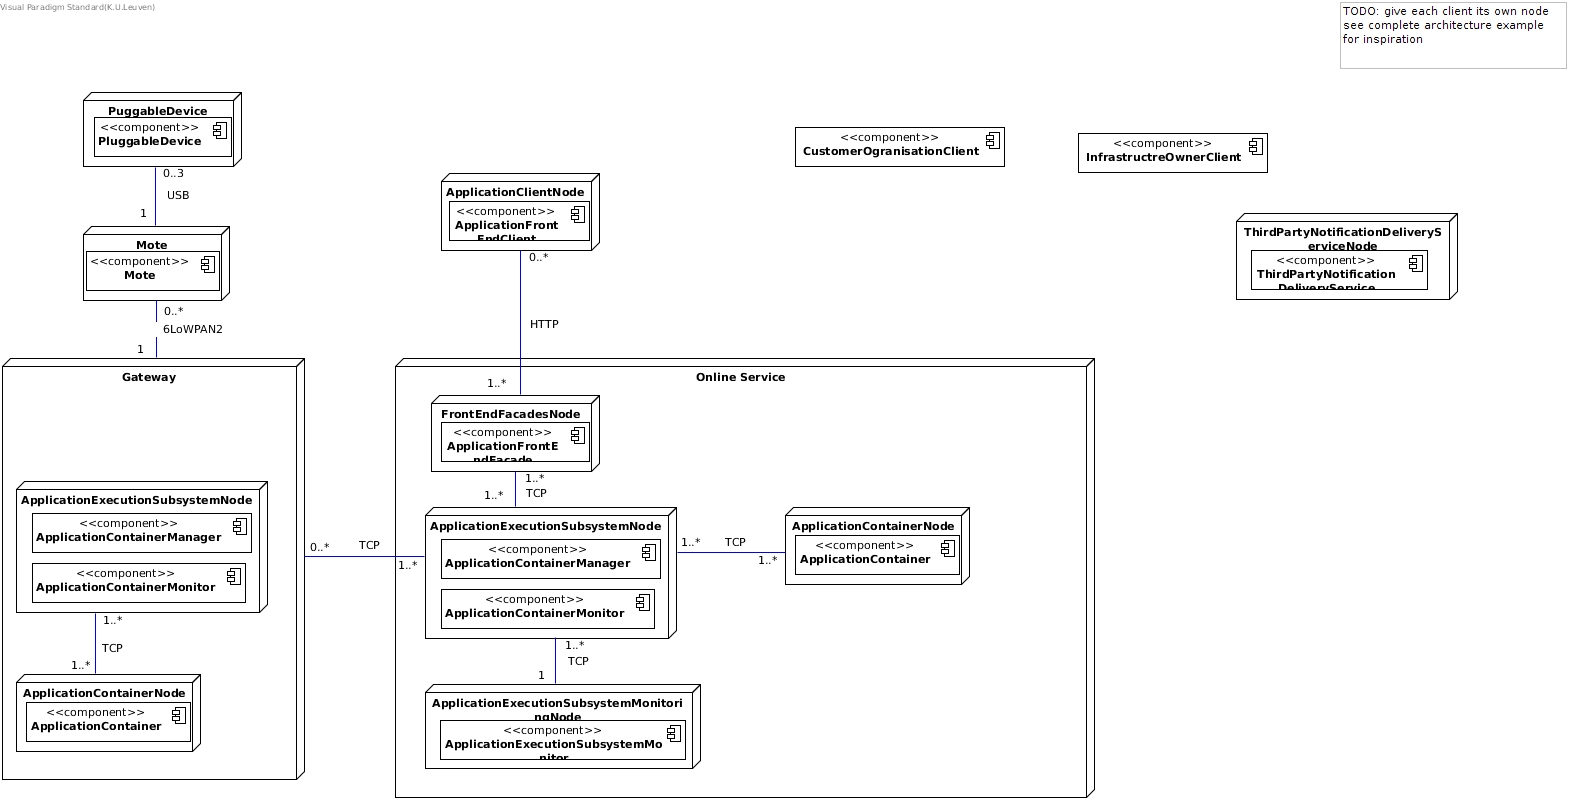
\includegraphics[width=\textwidth]{images/deployment-context}
            	\caption{Context diagram for the deployment view.}\label{fig:depl_context}
            \end{figure}

        \vfill
    \end{landscape}


\section{Primary diagram}
    The primary diagram for the deployment view is displayed in figure \ref{fig:depl_primary}.

    TODO: add references to "architectural decisions" where we made some choices related to deployment of components. \\

    \todoinline{
    The primary deployment diagram itself.
    This discussion on the parts of the deployment diagram which are crucial for
    achieving certain non-functional requirements, and any alternative deployments that you considered, should be in the architectural decisions chapter.
    }

    \begin{landscape}
        \centering
        \vspace*{\fill}

            \begin{figure}[!htp]
            	\centering
                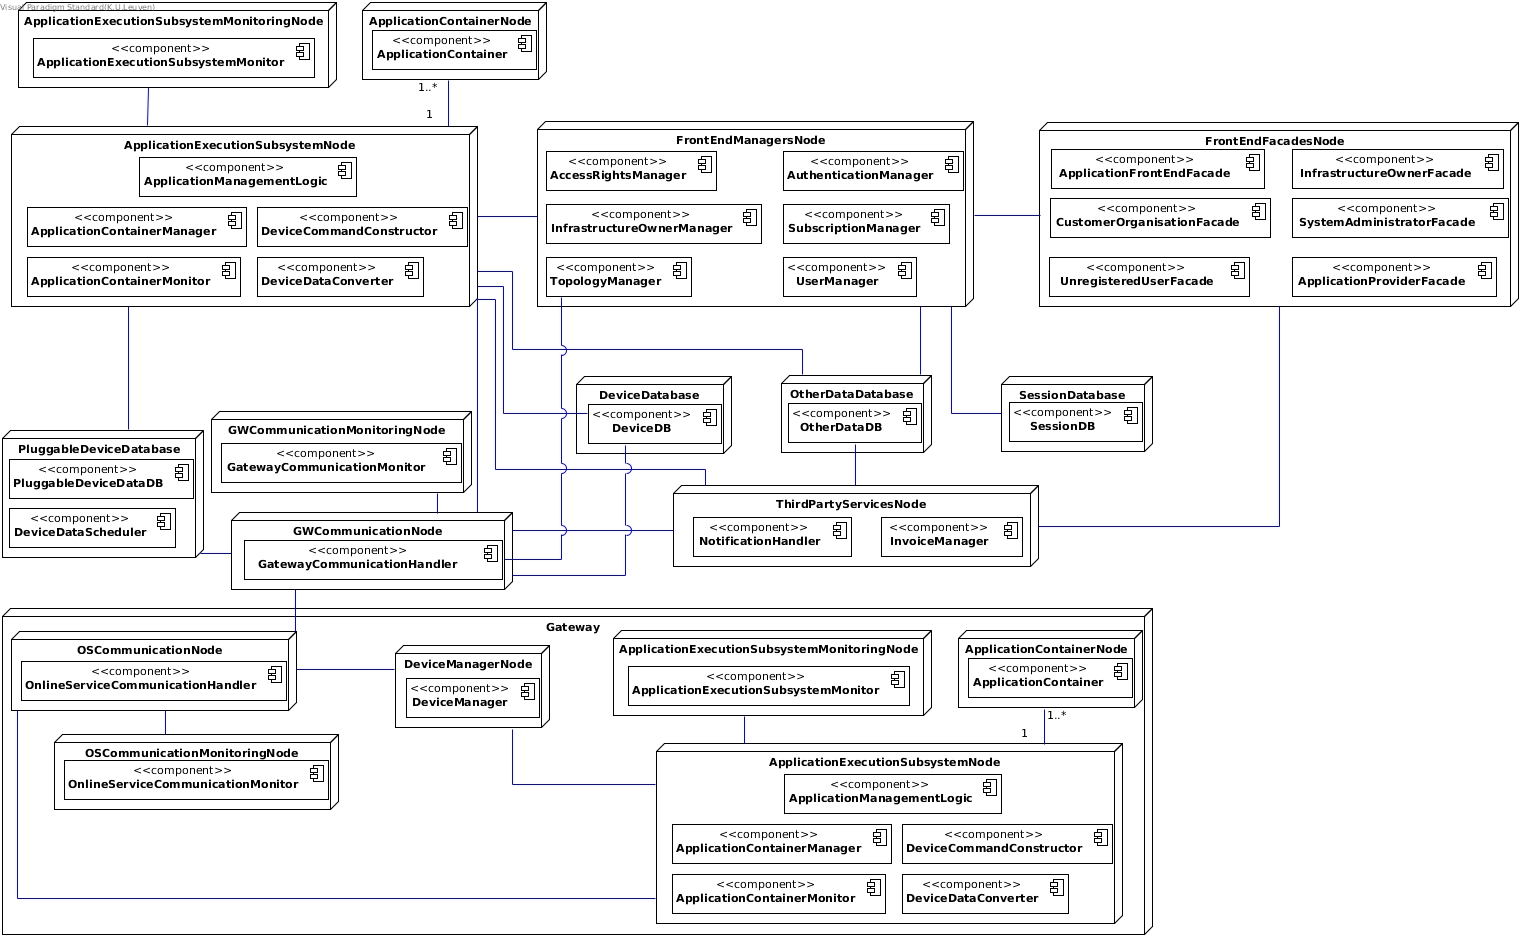
\includegraphics[width=\textwidth]{images/deployment-primary}
            	\caption{Primary diagram for the deployment view.}\label{fig:depl_primary}
            \end{figure}

        \vfill
    \end{landscape}
